\documentclass[a4paper]{article}
\usepackage{graphicx}
\usepackage{coqdoc}
\usepackage{amsmath}
\usepackage{amsthm}
\usepackage{amssymb}
\usepackage[all]{xy}
\usepackage{mathpartir}
\usepackage{tabto,calc}
\usepackage{onecolceurws}

\newcommand{\tto}{\twoheadrightarrow}
\newcommand{\ott}{\twoheadleftarrow}
\newcommand{\flavio}[1]{{\color{red}#1}}

\newcommand{\comm}[1]{\tabto{\CurrentLineWidth}\fbox{\begin{minipage}[t]{0.98\linewidth-\TabPrevPos} #1 \end{minipage}}}

\newtheorem{theorem}{Theorem}[section]
\newtheorem{definition}{Definition}[section]
\newtheorem{lemma}{Lemma}[section]

\title{A Formalization of the (Compositional) Z Property}

\author{
Flávio L. C. de Moura and Leandro O. Rezende\\ Dept. de Ciência da Computação\\
                Universidade de Brasília \\ flaviomoura@unb.br
}

\institution{}

\begin{document}
\maketitle

\begin{abstract}
  Rewriting theory is a well established model of computation
  equivalent to the Turing machines, and the most well known rewriting
  system is the $\lambda$-calculus. Confluence is an important and
  undecidable property related to the determinism of the computational
  process. Direct proofs of confluence are, in general, difficult to
  be done. Therefore, alternative characterizations of confluence can
  circumvent this difficulty for different contexts. This is the case
  of the so called Z property, which has been successfully used to
  prove confluence in several situations such as the
  $\lambda$-calculus with $\beta\eta$-reduction, extensions of the
  $\lambda$-calculus with explicit substitutions, the
  $\lambda\mu$-calculus, etc. In this work we present a direct and
  constructive proof that the Z property implies confluence.  In
  addition, we formalized our proof and an extension of the Z
  property, known as the Compositional Z, in the Coq proof assistant.
\end{abstract}
\vskip 32pt


\section{Introduction}

Confluence is an important and undecidable property concerning the
determinism of the computational process. This means that
independently of the choice of the evaluation path, the result is
always the same. In the particular case of Abstract Rewriting Systems
(ARS), which are the focus of this work, confluence can be beautifully
expressed by diagrams as we will see in the next section.

The contributions of this work are as follows:
\begin{itemize}
\item We present a proof that the Z property implies confluence,
  which is direct and constructive.
\item The proof that the Z property implies confluence is formalized
  in the Coq proof assistant. 
\item We formalize an extension of the Z property, known as
  compositional Z property, as presented in
  \cite{Nakazawa-Fujita2016}. The proofs are presented by interleaving
  Coq code followed by an explanation in English of the corresponding
  code. In this way, the annotations are done directly in the Coq
  files using the coqdoc annotation style. We believe that this
  approach is interesting for those that are not familiar with the Coq
  proof assistant because the Coq code followed by English
  explanations gives a good idea on how they relate to each
  other. This discipline also forces a better organization of the
  formalization and of the proofs so that the explanation in English
  is comprehensible.
\end{itemize}

\section{The Z property implies Confluence}

An ARS, say $(A,R)$, is a pair composed of a set $A$ and binary
relation over this set $R:A\times A$. Let $a,b\in A$. We write
$a\to_R b$ (or $R\ a\ b$ in the Coq syntax below) to denote that
$(a,b)\in R$, and in this case, we say that $a$ $R$-reduces to $b$ in
one step. The reflexive transitive closure of a relation
\coqdocvar{R}, written as $\tto_R$, is defined by the following
inference rules: \begin{mathpar} \inferrule*[Right={$(refl)$}]{~}{a
    \tto_R a} \and \inferrule*[Right={$(rtrans)$}]{a\to_R b \and b
    \tto_R c}{a \tto_R c} \end{mathpar} \noindent where $a,b$ and $c$
are universally quantified variables as explicitly stated in the
corresponding Coq definition: \begin{coqdoccode} \coqdocemptyline
  \coqdocnoindent \coqdockw{Inductive} \coqdocvar{refltrans}
  \{\coqdocvar{A}:\coqdockw{Type}\} (\coqdocvar{R}: \coqdocvar{Rel}
  \coqdocvar{A}) : \coqdocvar{A} \ensuremath{\rightarrow}
  \coqdocvar{A} \ensuremath{\rightarrow} \coqdockw{Prop} :=\coqdoceol
  \coqdocnoindent \ensuremath{|} \coqdocvar{refl}:
  \coqdockw{\ensuremath{\forall}} \coqdocvar{a},
  (\coqdocvar{refltrans} \coqdocvar{R}) \coqdocvar{a}
  \coqdocvar{a}\coqdoceol \coqdocnoindent \ensuremath{|}
  \coqdocvar{rtrans}: \coqdockw{\ensuremath{\forall}} \coqdocvar{a}
  \coqdocvar{b} \coqdocvar{c}, \coqdocvar{R} \coqdocvar{a}
  \coqdocvar{b} \ensuremath{\rightarrow} \coqdocvar{refltrans}
  \coqdocvar{R} \coqdocvar{b} \coqdocvar{c} \ensuremath{\rightarrow}
  \coqdocvar{refltrans} \coqdocvar{R} \coqdocvar{a}
  \coqdocvar{c}.\coqdoceol \coqdocemptyline
\end{coqdoccode}

The reflexive transitive closure of a relation is used to define
    the notion of confluence: no matter how the reduction is done, the
    result will always be the same. In other words, every divergence
    is joinable as stated by the following diagram:


    $\centerline{\xymatrix{ & a \ar@{->>}[dl] \ar@{->>}[dr] & \\ b
    \ar@{.>>}[dr] & & c \ar@{.>>}[dl] \\ & d & }}$


Formally, this means that if an expression $a$ can be reduced in two
different ways to $b$ and $c$, then there exists an expression $d$
such that both $b$ and $c$ reduce to $d$. The existential
quantification is expressed by the dotted lines in the diagram. This
notion is defined in the Coq system as follows: \begin{coqdoccode}
  \coqdocemptyline \coqdocnoindent \coqdockw{Definition}
  \coqdocvar{Confl} \{\coqdocvar{A}:\coqdockw{Type}\} (\coqdocvar{R}:
  \coqdocvar{Rel} \coqdocvar{A}) := \coqdockw{\ensuremath{\forall}}
  \coqdocvar{a} \coqdocvar{b} \coqdocvar{c}, (\coqdocvar{refltrans}
  \coqdocvar{R}) \coqdocvar{a} \coqdocvar{b} \ensuremath{\rightarrow}
  (\coqdocvar{refltrans} \coqdocvar{R}) \coqdocvar{a} \coqdocvar{c}
  \ensuremath{\rightarrow} (\coqdoctac{\ensuremath{\exists}}
  \coqdocvar{d}, (\coqdocvar{refltrans} \coqdocvar{R}) \coqdocvar{b}
  \coqdocvar{d} \ensuremath{\land} (\coqdocvar{refltrans}
  \coqdocvar{R}) \coqdocvar{c} \coqdocvar{d}).\coqdoceol
  \coqdocemptyline
\end{coqdoccode}

In \cite{dehornoy2008z}, V. van Oostrom gives a sufficient condition
for an ARS to be confluent. This condition is based on the \textit{Z
  Property} that is defined as follows:


\begin{definition} Let $(A,\to_R)$ be an ARS. A mapping $f:A \to A$ 
  satisfies the Z property for $\to_R$, if $a \to_R b$ implies
  $b \tto_R f a  \tto_R f b$, for any $a, b \in A$. 
\end{definition}

The name of the property comes from the following diagrammatic
representation of this definition:
    
\[ \xymatrix{ a \ar[r]_R & b \ar@{.>>}[dl]^R\\ f a \ar@{.>>}[r]_R & f
    b \\ } \]

If a function \coqdocvar{f} satisfies the Z property for $\to_R$ then
we say that \coqdocvar{f} is Z for $\to_R$, and the corresponding Coq
definition is given by the following predicate:

\begin{coqdoccode}
  \coqdocemptyline \coqdocnoindent \coqdockw{Definition}
  \coqdocvar{f\_is\_Z} \{\coqdocvar{A}:\coqdockw{Type}\}
  (\coqdocvar{R}: \coqdocvar{Rel} \coqdocvar{A}) (\coqdocvar{f}:
  \coqdocvar{A} \ensuremath{\rightarrow} \coqdocvar{A}) :=
  \coqdockw{\ensuremath{\forall}} \coqdocvar{a} \coqdocvar{b},
  \coqdocvar{R} \coqdocvar{a} \coqdocvar{b} \ensuremath{\rightarrow}
  ((\coqdocvar{refltrans} \coqdocvar{R}) \coqdocvar{b} (\coqdocvar{f}
  \coqdocvar{a}) \ensuremath{\land} (\coqdocvar{refltrans}
  \coqdocvar{R}) (\coqdocvar{f} \coqdocvar{a}) (\coqdocvar{f}
  \coqdocvar{b})).\coqdoceol \coqdocemptyline
\end{coqdoccode}

Alternatively, an ARS $(A,\to_R)$ satisfies the Z property if there
exists a mapping $f:A \to A$ such that $f$ is Z for $\to_R$:

\begin{coqdoccode}
  \coqdocemptyline \coqdocnoindent \coqdockw{Definition}
  \coqdocvar{Z\_prop} \{\coqdocvar{A}:\coqdockw{Type}\}
  (\coqdocvar{R}: \coqdocvar{Rel} \coqdocvar{A}) :=
  \coqdoctac{\ensuremath{\exists}} \coqdocvar{f}:\coqdocvar{A}
  \ensuremath{\rightarrow} \coqdocvar{A},
  \coqdockw{\ensuremath{\forall}} \coqdocvar{a} \coqdocvar{b},
  \coqdocvar{R} \coqdocvar{a} \coqdocvar{b} \ensuremath{\rightarrow}
  ((\coqdocvar{refltrans} \coqdocvar{R}) \coqdocvar{b} (\coqdocvar{f}
  \coqdocvar{a}) \ensuremath{\land} (\coqdocvar{refltrans}
  \coqdocvar{R}) (\coqdocvar{f} \coqdocvar{a}) (\coqdocvar{f}
  \coqdocvar{b})).\coqdoceol \coqdocemptyline
\end{coqdoccode}

The first contribution of this work is a constructive proof of the
fact that the Z property implies confluence. Our proof uses nested
induction, and hence it differs from the one in \cite{kes09} (that
follows \cite{dehornoy2008z}) and the one in \cite{zproperty} in the
sense that it does not rely on the analyses of whether a term is in
normal form or not, avoiding the necessity of the law of the excluded
middle. As a result, we have an elegant inductive proof of the fact
that if an ARS satisfies the Z property then it is confluent. This
proof is formalized in the Coq proof assistant, and the whole
formalization is available in a GitHub
repository\footnote{\label{fn:github}\url{https://github.com/flaviodemoura/Zproperty}}. The
following proof is the first contribution of this work:
\begin{theorem}\cite{dehornoy2008z}
  If there exists a mapping satisfying the Z property for an abstract
  rewriting system, then it is confluent.
\end{theorem}
\begin{proof}
  Let $(A,\to)$ be an ARS, and $f: A \to A$ a function that is Z for
  $\to$. Let $b \ott a \tto c$ be an arbitrary divergence. The proof
  proceeds by induction on the reduction $a \tto b$, and according to
  the definition of the reflexive transitive closure of a relation, we
  have two cases: in the first case, $a=b$ and we are done. Otherwise,
  $a \to b' \tto b$ for some term $b'$. We now want to proceed by
  induction on the reduction $a \tto c$, for which the first case is
  also trivial, but the other case cannot be proved using the last
  generated induction hypothesis. In fact, suppose that
  $a \to c' \tto c$, for some term $c'$. The induction hypothesis now
  refers to $c'$ and the hypothesis $a \to b'$ is transformed in the
  condition $c' \to b'$, which is not provable, therefore we get
  stuck. The way to circumvent this problem is by reorganizing the
  proof context by removing the hypothesis $a \to b$ before starting
  the inner induction on $a \tto c$. The Z property will allow this
  reorganization because the hypothesis $a \to b$ will be replaced by
  $b \tto (f\ a)$ that is straightforward from the Z property, and by
  $a \tto (f\ a)$ that is obtained from the transitivity of $\to$. The
  new context allows us to proceed by induction on the reduction
  $a \tto c$, as expected because the hypothesis $a \tto (f\ a)$ is
  transformed in the condition $c' \tto (f\ c')$ which can be proved
  using the Z property. The details of the whole proof can be found in
  the technical report\textsuperscript{\ref{fn:github}}.
\end{proof}
  
The interesting point of the above proof is that it reveals the
difficulties that are usually made invisible by graphical proofs. In
the next section, we present the formalization of an extension of the
Z property known as Compositional Z.

\section{An extension of the Z property: Compositional Z}

In this section we present a formalization of the
\textit{Compositional Z}, as presented in \cite{Nakazawa-Fujita2016},
which is an interesting property because it allows a kind of modular
approach to the Z property when the reduction relation can be split
into smaller relations. More precisely, given an ARS $(A,\to_R)$, one
must be able to decompose the relation $\to_R$ into two parts, say
$\to_1$ and $\to_2$ such that $\to_R = \to_1\cup \to_2$. This kind of
decomposition can be done in several interesting situations such as
the $\lambda$-calculus with $\beta\eta$-reduction\cite{Ba84},
extensions of the $\lambda$-calculus with explicit
substitutions\cite{accl91}, the $\lambda\mu$-calculus\cite{Parigot92},
etc. But before presenting the full definition of the Compositional Z,
we need to define the \textit{weak Z property}:

\begin{figure}[h] \centering \[ \xymatrix{ a \ar[r]_R & b
      \ar@{.>>}[dl]^x\\ f(a) \ar@{.>>}[r]_x & f(b) \\ } \]
  \caption{The weak Z property}\label{fig:weakZ}
\end{figure}

\begin{definition} Let $(A,\to_R)$ be an ARS and $\to_R'$ be another
  relation on $A$. A mapping $f$ satisfies the {\it weak Z property}
  for $\to_R$ by $\to_R'$ if $a\to_R b$ implies $b \tto_R' f(a)$ and
  $f(a) \tto_R' f(b)$ (cf. Figure \ref{fig:weakZ}). Therefore, a
  mapping $f$ satisfies the Z property for $\to_R$ if it satisfies the
  weak Z property by itself.
\end{definition}

When $f$ satisfies the weak Z property, we also say that $f$ is weakly
Z, and the corresponding definition in Coq is given as
follows: \begin{coqdoccode} \coqdocemptyline \coqdocnoindent
  \coqdockw{Definition} \coqdocvar{f\_is\_weak\_Z} \{\coqdocvar{A}\}
  (\coqdocvar{R} \coqdocvar{R'}: \coqdocvar{Rel} \coqdocvar{A})
  (\coqdocvar{f}: \coqdocvar{A} \ensuremath{\rightarrow}
  \coqdocvar{A}) := \coqdockw{\ensuremath{\forall}} \coqdocvar{a}
  \coqdocvar{b}, \coqdocvar{R} \coqdocvar{a} \coqdocvar{b}
  \ensuremath{\rightarrow} ((\coqdocvar{refltrans} \coqdocvar{R'})
  \coqdocvar{b} (\coqdocvar{f} \coqdocvar{a}) \ensuremath{\land}
  (\coqdocvar{refltrans} \coqdocvar{R'}) (\coqdocvar{f} \coqdocvar{a})
  (\coqdocvar{f} \coqdocvar{b})).\coqdoceol \coqdocemptyline
\end{coqdoccode}

The compositional Z is then defined as follows:

\begin{definition}\cite{Nakazawa-Fujita2016}
  Let $(A,\to)$ be an ARS such that $\to = \to_1 \cup \to_2$. The
  $(A,\to)$ satisfies the compositional Z if there exist mappings
  $f_1:A \to A$ and $f_2:A \to A$ such that:
  \begin{enumerate}
  \item $f_1$ is Z for $\to_1$;
  \item $a \to_1 b$ implies $f_2\ a \tto f_2\ b$;
  \item $a \tto f_2\ a$ holds for any $a \in Im(f_1)$, and
  \item $f_2\circ f_1$ is weakly Z for $\to_2$ by $\to$.
  \end{enumerate}
\end{definition}

The corresponding definition in the Coq proof assistant is below,
where the composition of $f_2\circ f_1$ is written as \coqdocvar{f2}
\# \coqdocvar{f1}, i.e. (\coqdocvar{f2} \# \coqdocvar{f1})$x$ =
\coqdocvar{f2}(\coqdocvar{f1}\ $x$), and the union $\to_1 \cup \to_2$
written as R1 !\_! R2.

\begin{coqdoccode}
  \coqdocemptyline \coqdocnoindent \coqdockw{Definition}
  \coqdocvar{Z\_comp} \{\coqdocvar{A}:\coqdockw{Type}\} (\coqdocvar{R}
  :\coqdocvar{Rel} \coqdocvar{A}) := \coqdoctac{\ensuremath{\exists}}
  (\coqdocvar{R1} \coqdocvar{R2}: \coqdocvar{Rel} \coqdocvar{A})
  (\coqdocvar{f1} \coqdocvar{f2}: \coqdocvar{A}
  \ensuremath{\rightarrow} \coqdocvar{A}), \coqdocvar{R} =
  (\coqdocvar{R1} !\coqdocvar{\_}! \coqdocvar{R2}) \ensuremath{\land}
  \coqdocvar{f\_is\_Z} \coqdocvar{R1} \coqdocvar{f1}
  \ensuremath{\land} (\coqdockw{\ensuremath{\forall}} \coqdocvar{a}
  \coqdocvar{b}, \coqdocvar{R1} \coqdocvar{a} \coqdocvar{b}
  \ensuremath{\rightarrow} (\coqdocvar{refltrans} \coqdocvar{R})
  (\coqdocvar{f2} \coqdocvar{a}) (\coqdocvar{f2} \coqdocvar{b}))
  \ensuremath{\land} (\coqdockw{\ensuremath{\forall}} \coqdocvar{a}
  \coqdocvar{b}, \coqdocvar{b} = \coqdocvar{f1} \coqdocvar{a}
  \ensuremath{\rightarrow} (\coqdocvar{refltrans} \coqdocvar{R})
  \coqdocvar{b} (\coqdocvar{f2} \coqdocvar{b})) \ensuremath{\land}
  (\coqdocvar{f\_is\_weak\_Z} \coqdocvar{R2} \coqdocvar{R}
  (\coqdocvar{f2} \# \coqdocvar{f1})).\coqdoceol \coqdocemptyline
  \coqdocemptyline
\end{coqdoccode}

The next theorem is proved by presenting the Coq proof interleaved with natural language explaining the corresponding Coq steps. As an immediate consequence of this theorem, we get the confluence of the reduction relation $R$.

\begin{coqdoccode}
\coqdocemptyline
\coqdocnoindent
\coqdockw{Theorem} \coqdocvar{Z\_comp\_implies\_Z\_prop} \{\coqdocvar{A}:\coqdockw{Type}\}: \coqdockw{\ensuremath{\forall}} (\coqdocvar{R} :\coqdocvar{Rel} \coqdocvar{A}), \coqdocvar{Z\_comp} \coqdocvar{R} \ensuremath{\rightarrow} \coqdocvar{Z\_prop} \coqdocvar{R}.\coqdoceol
\coqdocnoindent
\coqdockw{Proof}.\coqdoceol
\coqdocindent{1.00em}
\coqdoctac{intros} \coqdocvar{R} \coqdocvar{H}. \end{coqdoccode}
\comm{Let $R$ be a relation over $A$, and $H$ the
      hypothesis that $R$ satisfies the compositional Z.} \begin{coqdoccode}
\coqdocemptyline
\coqdocindent{1.00em}
\coqdoctac{unfold} \coqdocvar{Z\_prop}. \coqdoctac{unfold} \coqdocvar{Z\_comp} \coqdoctac{in} \coqdocvar{H}. \coqdoctac{destruct} \coqdocvar{H} \coqdockw{as}\coqdoceol
\coqdocindent{1.00em}
[ \coqdocvar{R1} [ \coqdocvar{R2} [\coqdocvar{f1} [\coqdocvar{f2} [\coqdocvar{Hunion} [\coqdocvar{H1} [\coqdocvar{H2} [\coqdocvar{H3} \coqdocvar{H4}]]]]]]]]. \end{coqdoccode}
\comm{After unfolding the definitions $Z\_prop$ and $Z\_comp$, we need to prove the existence of a map, say $f$, that is Z as shown by the current proof context:
      \newline

      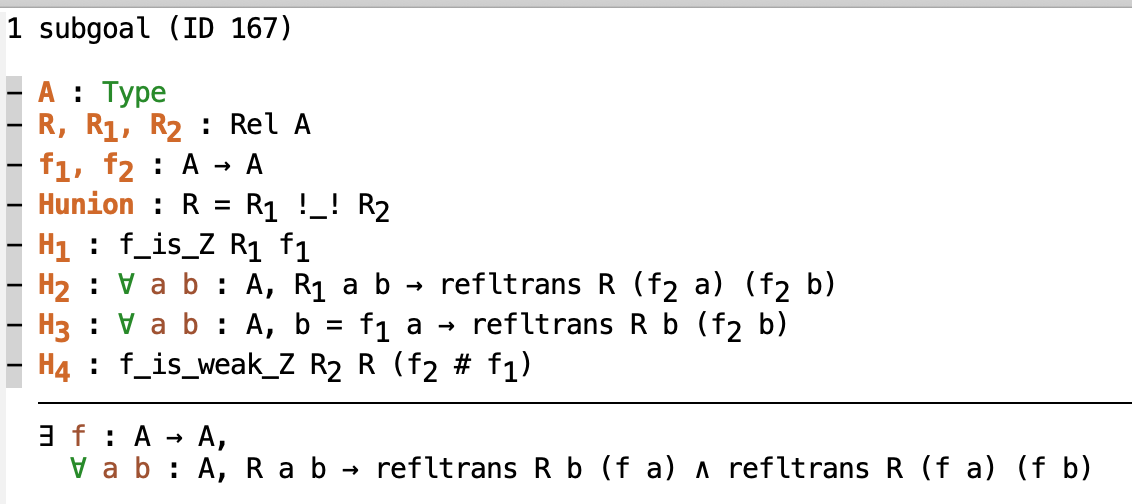
\includegraphics[scale=0.4]{figs/fig8.png} } \begin{coqdoccode}
\coqdocemptyline
\coqdocindent{1.00em}
\coqdoctac{\ensuremath{\exists}} (\coqdocvar{f2} \# \coqdocvar{f1}). \end{coqdoccode}
\comm{We will prove that the composition of f2 with f1 is Z.} \begin{coqdoccode}
\coqdocemptyline
\coqdocindent{1.00em}
\coqdoctac{intros} \coqdocvar{a} \coqdocvar{b} \coqdocvar{HR}. \end{coqdoccode}
\comm{Let $a$ and $b$ be elements of $A$, and suppose
  that $a$ $R$-reduces to $b$ in one step, i.e. that $a \to_R b$ and
  call $HR$ this hypothesis.} \begin{coqdoccode}
\coqdocemptyline
\coqdocindent{1.00em}
\coqdoctac{inversion} \coqdocvar{Hunion}; \coqdoctac{subst}. \coqdoctac{clear} \coqdocvar{H}. \coqdoctac{inversion} \coqdocvar{HR}; \coqdoctac{subst}. \end{coqdoccode}
\comm{Since
  $R$ is the union of $R1$ and $R2$, one has that $a$ reduces to $b$
  in one step via either $R1$ or $R2$. Therefore, there are two cases
  to consider:} \begin{coqdoccode}
\coqdocemptyline
\coqdocindent{1.00em}
- \coqdoctac{split}. \end{coqdoccode}
\comm{Firstly, suppose that $a$ $R1$-reduces in one step to
    $b$, i.e. $a \to_{R1} b$.} \begin{coqdoccode}
\coqdocemptyline
\coqdocindent{2.00em}
+ \coqdoctac{apply} \coqdocvar{refltrans\_composition} \coqdockw{with} (\coqdocvar{f1} \coqdocvar{a}). \end{coqdoccode}
\comm{In order to prove
    that $b \tto_R (f_2 (f_1\ a))$, we first need to show that $b
    \tto_{R1} (f_1\ a)$, and then that $(f_1\ a) \tto_R (f_2 (f_1\ a))$.} \begin{coqdoccode}
\coqdocemptyline
\coqdocindent{3.00em}
\ensuremath{\times} \coqdoctac{apply} \coqdocvar{H1} \coqdoctac{in} \coqdocvar{H}. \coqdoctac{destruct} \coqdocvar{H}. \coqdoctac{apply} \coqdocvar{refltrans\_union}; \coqdoctac{assumption}. \end{coqdoccode}
    \comm{The proof of $b \tto_{R1} (f_1\ a)$ is done from the fact that $f_1$
    is Z for $R1$.} \begin{coqdoccode}
\coqdocemptyline
\coqdocindent{3.00em}
\ensuremath{\times} \coqdoctac{apply} \coqdocvar{H3} \coqdockw{with} \coqdocvar{a}; \coqdoctac{reflexivity}. \end{coqdoccode}
\comm{The proof that $(f_1\ a)
    \tto_R (f_2 (f_1\ a))$ is a direct consequence of the hypothesis
    $H3$.} \begin{coqdoccode}
\coqdocemptyline
\coqdocindent{2.00em}
+ \coqdoctac{apply} \coqdocvar{H1} \coqdoctac{in} \coqdocvar{H}. \coqdoctac{destruct} \coqdocvar{H}. \coqdoctac{clear} \coqdocvar{H} \coqdocvar{HR}. \coqdoctac{unfold} \coqdocvar{comp}. \end{coqdoccode}
\comm{The
    proof that $(f_2 (f_1\ a))$ $R$-reduces to $(f_2 (f_1\ b))$ is
    more tricky. Initially, note that, since $a \to_{R1} b$ then we
    get that $(f_1\ a) \tto_{R1} (f_1\ b)$ by the Z property.} \begin{coqdoccode}
\coqdocemptyline
\coqdocindent{3.00em}
\coqdoctac{induction} \coqdocvar{H0}. \end{coqdoccode}
\comm{Now, the goal can be obtained from $H2$ as
      long as $(f_1\ a) \to_{R1} (f_1\ b)$, but from the hypothesis
      $H0$ we have that $(f_1\ a) \tto_{R1} (f_1\ b)$. Therefore, we
      proceed by induction on $H0$.} \begin{coqdoccode}
\coqdocemptyline
\coqdocindent{3.00em}
\ensuremath{\times} \coqdoctac{apply} \coqdocvar{refl}. \end{coqdoccode}
\comm{The reflexive case is trivial because $a$ and
        $b$ are equal.} \begin{coqdoccode}
\coqdocemptyline
\coqdocindent{3.00em}
\ensuremath{\times} \coqdoctac{apply} \coqdocvar{refltrans\_composition}\coqdoceol
\coqdocindent{7.00em}
\coqdoceol
\coqdocindent{4.00em}
\coqdockw{with} (\coqdocvar{f2} \coqdocvar{b0}). \end{coqdoccode}
\comm{In the transitive case, we have that $(f_1\ a)$ $R1$-reduces to
        $(f_1\ b)$ in at least one step. The current proof context is
        as follows, up to renaming of variables:

        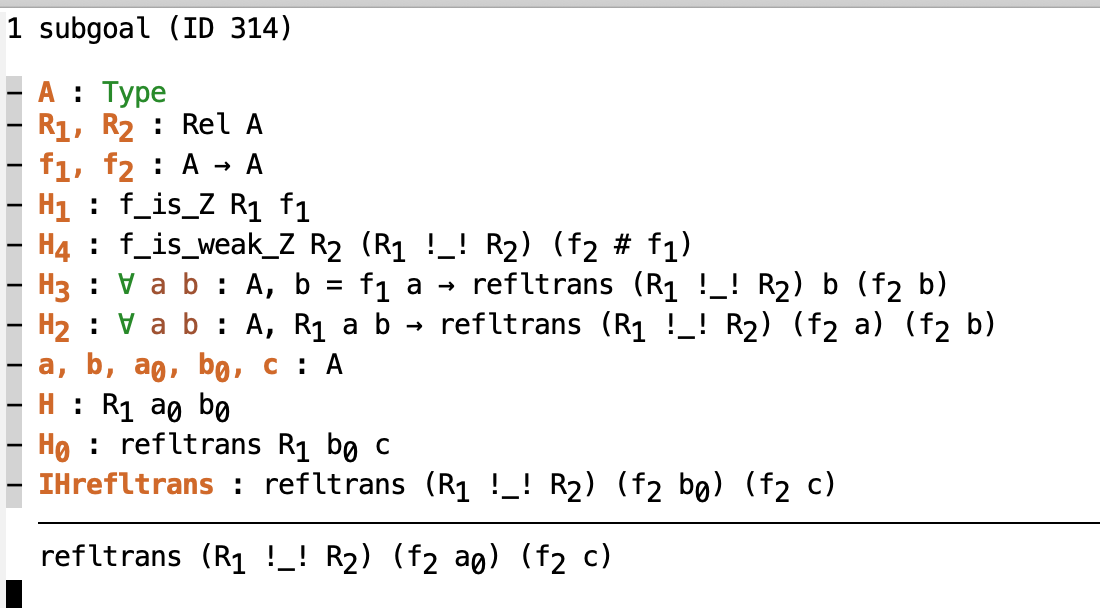
\includegraphics[scale=0.5]{figs/fig9.png}

      Therefore, there exists some element $b0$ such that $a0\to_{R1}
      b0$ and $b0 \tto_{R1} c$ and we need to prove that $(f_2\ a0)
      \tto_{R1\cup R2} (f_2\ c)$. This can be done in two steps using
      the transitivity of $\tto_{R1\cup R2}$ taking $(f_2\ b0)$ as the
      intermediary term.} \begin{coqdoccode}
\coqdocemptyline
\coqdocindent{4.00em}
** \coqdoctac{apply} \coqdocvar{H2}; \coqdoctac{assumption}. \end{coqdoccode}
\comm{The first subgoal is then $(f_2\
           a0)\tto_{(R1 \cup R2)} (f_2\ b0)$ that is proved by
           hypothesis $H2$.} \begin{coqdoccode}
\coqdocemptyline
\coqdocindent{4.00em}
** \coqdoctac{assumption}. \end{coqdoccode}
\comm{And the second subgoal $(f_2\ b0) \tto_{(R1
           \cup R2)} (f_2\ c)$ is proved by the induction
           hypothesis.} \begin{coqdoccode}
\coqdocemptyline
\coqdocindent{1.00em}
- \coqdoctac{apply} \coqdocvar{H4}; \coqdoctac{assumption}. \end{coqdoccode}
\comm{Finally, when $a$ $R2$-reduces in one
    step to $b$ one concludes the proof using the assumption that
    $(f_2 \circ f_1)$ is weak Z.} \begin{coqdoccode}
\coqdocemptyline
\coqdocnoindent
\coqdockw{Qed}.\coqdoceol
\coqdocemptyline
\end{coqdoccode}

Rewriting Systems with equations is another interesting and
non-trivial topic \cite{winkler89,terese03}. The confluence of
rewriting systems with an equivalence relation can also be proved by a
variant of the compositional Z, known as Z property
modulo~\cite{AK12b}. We define the predicate \coqdocvar{Z\_comp\_eq}
corresponding to the Z property modulo, and prove directly
that if \coqdocvar{Z\_comp\_eq} holds for a relation \coqdocvar{R}
then \coqdocvar{Zprop} \coqdocvar{R} also holds.

\begin{coqdoccode}
\coqdocemptyline
\coqdocnoindent
\coqdockw{Definition} \coqdocvar{Z\_comp\_eq} \{\coqdocvar{A}:\coqdockw{Type}\} (\coqdocvar{R} :\coqdocvar{Rel} \coqdocvar{A}) := \coqdoctac{\ensuremath{\exists}} (\coqdocvar{R1} \coqdocvar{R2}: \coqdocvar{Rel} \coqdocvar{A}) (\coqdocvar{f1} \coqdocvar{f2}: \coqdocvar{A} \ensuremath{\rightarrow} \coqdocvar{A}), \coqdocvar{R} = (\coqdocvar{R1} !\coqdocvar{\_}! \coqdocvar{R2}) \ensuremath{\land} (\coqdockw{\ensuremath{\forall}} \coqdocvar{a} \coqdocvar{b}, \coqdocvar{R1} \coqdocvar{a} \coqdocvar{b} \ensuremath{\rightarrow} (\coqdocvar{f1} \coqdocvar{a}) = (\coqdocvar{f1} \coqdocvar{b})) \ensuremath{\land} (\coqdockw{\ensuremath{\forall}} \coqdocvar{a}, (\coqdocvar{refltrans} \coqdocvar{R1}) \coqdocvar{a} (\coqdocvar{f1} \coqdocvar{a})) \ensuremath{\land} (\coqdockw{\ensuremath{\forall}} \coqdocvar{b} \coqdocvar{a}, \coqdocvar{a} = \coqdocvar{f1} \coqdocvar{b} \ensuremath{\rightarrow} (\coqdocvar{refltrans} \coqdocvar{R}) \coqdocvar{a} (\coqdocvar{f2} \coqdocvar{a})) \ensuremath{\land} (\coqdocvar{f\_is\_weak\_Z} \coqdocvar{R2} \coqdocvar{R} (\coqdocvar{f2} \# \coqdocvar{f1})).\coqdoceol
\coqdocemptyline
\coqdocnoindent
\coqdockw{Lemma} \coqdocvar{Z\_comp\_eq\_implies\_Z\_prop} \{\coqdocvar{A}:\coqdockw{Type}\}: \coqdockw{\ensuremath{\forall}} (\coqdocvar{R} : \coqdocvar{Rel} \coqdocvar{A}), \coqdocvar{Z\_comp\_eq} \coqdocvar{R} \ensuremath{\rightarrow} \coqdocvar{Z\_prop} \coqdocvar{R}.\coqdoceol
\coqdocnoindent
\coqdockw{Proof}.\coqdoceol
\coqdocindent{1.00em}
\coqdoctac{intros} \coqdocvar{R} \coqdocvar{Heq}. \coqdoctac{unfold} \coqdocvar{Z\_comp\_eq} \coqdoctac{in} \coqdocvar{Heq}. \end{coqdoccode}
\comm{Let $R$ be a relation
  and suppose that $R$ satisfies the predicate $Z\_comp\_eq$.} \begin{coqdoccode}
\coqdocemptyline
\coqdocindent{1.00em}
\coqdoctac{destruct} \coqdocvar{Heq} \coqdockw{as} [\coqdocvar{R1} [\coqdocvar{R2} [\coqdocvar{f1} [\coqdocvar{f2} [\coqdocvar{Hunion} [\coqdocvar{H1} [\coqdocvar{H2} [\coqdocvar{H3} \coqdocvar{H4}]]]]]]]]. \end{coqdoccode}
\comm{Call $Hi$ the $i$th hypothesis, $i\in\{1,2,3,4\}$.}
\begin{coqdoccode}
\coqdocemptyline
\coqdocindent{1.00em}
\coqdoctac{unfold} \coqdocvar{Z\_prop}. \coqdoctac{\ensuremath{\exists}} (\coqdocvar{f2} \# \coqdocvar{f1}). \end{coqdoccode}
\comm{From the definition of the
  predicate $Z\_prop$, we need to find a map, say $f$ that is Z. Let
  $(f_2 \circ f_1)$ be such map.}  \begin{coqdoccode}
\coqdocemptyline
\coqdocindent{1.00em}
\coqdoctac{intros} \coqdocvar{a} \coqdocvar{b} \coqdocvar{Hab}. \end{coqdoccode}
\comm{In order to prove that $(f_2 \circ f_1)$ is Z,
  let $a$ and $b$ be arbitrary elements of type $A$, and $Hab$ be the
  hypothesis that $a \to_{R} b$.} \begin{coqdoccode}
\coqdocemptyline
\coqdocindent{1.00em}
\coqdoctac{inversion} \coqdocvar{Hunion}; \coqdoctac{subst}; \coqdoctac{clear} \coqdocvar{H}. \coqdoctac{inversion} \coqdocvar{Hab}; \coqdoctac{subst}; \coqdoctac{clear} \coqdocvar{Hab}. \end{coqdoccode}
  \comm{Since $a$ $R$-reduces in one step to $b$ and $R$ is the union of the
  relations $R1$ and $R2$ then we consider two cases:} \begin{coqdoccode}
\coqdocemptyline
\coqdocindent{1.00em}
- \coqdoctac{unfold} \coqdocvar{comp}; \coqdoctac{split}. \end{coqdoccode}
\comm{The first case is when $a \to_{R1}
    b$. This is equivalent to say that $f_2 \circ f_1$ is weak Z for
    $R1$ by $R1 \cup R2$.} \begin{coqdoccode}
\coqdocemptyline
\coqdocindent{2.00em}
+ \coqdoctac{apply} \coqdocvar{refltrans\_composition} \coqdockw{with} (\coqdocvar{f1} \coqdocvar{b}). \end{coqdoccode}
\comm{Therefore, we first
    prove that $b \tto_{(R1\cup R2)} (f_2 (f_1\ a))$, which can be
    reduced to $b \tto_{(R1\cup R2)} (f_1\ b)$ and $(f_1\ b)
    \tto_{(R1\cup R2)} (f_2 (f_1\ a))$ by the transitivity of
    $refltrans$.} \begin{coqdoccode}
\coqdocemptyline
\coqdocindent{3.00em}
\ensuremath{\times} \coqdoctac{apply} \coqdocvar{refltrans\_union}. \coqdoctac{apply} \coqdocvar{H2}. \end{coqdoccode}
\comm{From hypothesis $H2$, we
        know that $a \tto_{R1} (f_1\ a)$ for all $a$, and hence
        $a\tto_{(R1\cup R2)} (f_1\ a)$ and we conclude.} \begin{coqdoccode}
\coqdocemptyline
\coqdocindent{3.00em}
\ensuremath{\times} \coqdoctac{apply} \coqdocvar{H1} \coqdoctac{in} \coqdocvar{H}. \coqdoctac{rewrite} \coqdocvar{H}. \coqdoctac{apply} \coqdocvar{H3} \coqdockw{with} \coqdocvar{b}; \coqdoctac{reflexivity}. \end{coqdoccode}
        \comm{The proof that $(f_1\ b)\tto_{(R1\cup R2)} (f_2 (f_1\ a))$ is
        exactly the hypothesis $H3$.} \begin{coqdoccode}
\coqdocemptyline
\coqdocindent{2.00em}
+ \coqdoctac{apply} \coqdocvar{H1} \coqdoctac{in} \coqdocvar{H}. \coqdoctac{rewrite} \coqdocvar{H}. \coqdoctac{apply} \coqdocvar{refl}. \end{coqdoccode}
\comm{The proof that $(f_2
    (f_1\ a)) \tto_{(R1\cup R2)} (f_2 (f_1\ b))$ is done using the
    reflexivity of $refltrans$ because $(f_2 (f_1\ a)) = (f_2 (f_1\
    b))$ by hypothesis $H1$.} \begin{coqdoccode}
\coqdocemptyline
\coqdocindent{1.00em}
- \coqdoctac{apply} \coqdocvar{H4}; \coqdoctac{assumption}. \end{coqdoccode}
\comm{When $a \to_{R2} b$ then we are done by
    hypothesis $H4$.} \begin{coqdoccode}
\coqdocemptyline
\coqdocnoindent
\coqdockw{Qed}.\coqdoceol
\coqdocemptyline
\end{coqdoccode}

\section{Conclusion, Related Work and Future Work}

In this work we presented a constructive proof that the Z property
implies confluence, and this proof was formalized in the Coq proof
assistant\footnote{The corresponding files are available at
  \url{https://github.com/flaviodemoura/Zproperty}}.  Moreover, our
formalization includes an extension of the Z property, known as
compositional Z property, as presented in \cite{Nakazawa-Fujita2016}.

The Z property was presented by V. van Oostrom as a sufficient
condition for an ARS to be confluent~\cite{zproperty}, and since then
has been used to prove confluence in different contexts such as the
$\lambda$-calculus with $\beta\eta$-reduction, extensions of the
$\lambda$-calculus with explicit substitutions and the
$\lambda\mu$-calculus. In \cite{zproperty}, B. Felgenhauer
et.al. formalized the Z property in Isabelle/HOL via
semiconfluence. In \cite{vanoostrom:LIPIcs.FSCD.2021.24}, the
flexibility and applicability of the Z property is shown to prove
confluence and normalisation based on a syntax-free version of the
classical notion of development

As future work, this formalization will be used to prove the
confluence property of calculi with explicit substitutions using
different approaches such as nominal and locally nameless
representations.

\flavio{nominal and lnr for lx. checking missing biblio (oostrom 21)}

\bibliographystyle{alpha} 
\bibliography{references2}
%inline the .bbl file directly for mailing to authors.

\end{document}

